%settings are located in begin_settins.tex and end_settings.tex files -> do not remove the files!
%iso-8859-2 encoding
%%% Hlavní soubor. Zde se definují základní parametry a odkazuje se na ostatní části. %%%

%% Verze pro jednostranný tisk:
% Okraje: levý 40mm, pravý 25mm, horní a dolní 25mm
% (ale pozor, LaTeX si sám přidává 1in)
\documentclass[12pt,a4paper]{report}
\setlength\textwidth{145mm}
\setlength\textheight{247mm}
\setlength\oddsidemargin{15mm}
\setlength\evensidemargin{15mm}
\setlength\topmargin{0mm}
\setlength\headsep{0mm}
\setlength\headheight{0mm}
\usepackage[utf8]{inputenc}

%% Ostatní balíčky
\usepackage{graphicx}
\usepackage{amsthm}
\usepackage{listings}

%% Balíček hyperref, kterým jdou vyrábět klikací odkazy v PDF,
%% ale hlavně ho používáme k uložení metadat do PDF (včetně obsahu).
%% POZOR, nezapomeňte vyplnit jméno práce a autora.
\usepackage[ps2pdf,unicode]{hyperref}   % Musí být za všemi ostatními balíčky
\hypersetup{pdftitle=Data Warehouse Milestone}
\hypersetup{pdfauthor=Ondrej Platek and Peteris Nikiforovs}

%%% Drobné úpravy stylu

% Tato makra přesvědčují mírně ošklivým trikem LaTeX, aby hlavičky kapitol
% sázel příčetněji a nevynechával nad nimi spoustu místa. Směle ignorujte.
\makeatletter
\def\@makechapterhead#1{
  {\parindent \z@ \raggedright \normalfont
   \Huge\bfseries \thechapter. #1
   \par\nobreak
   \vskip 20\p@
}}
\def\@makeschapterhead#1{
  {\parindent \z@ \raggedright \normalfont
   \Huge\bfseries #1
   \par\nobreak
   \vskip 20\p@
}}
\makeatother

% Toto makro definuje kapitolu, která není očíslovaná, ale je uvedena v obsahu.
\def\chapwithtoc#1{
\chapter*{#1}
\addcontentsline{toc}{chapter}{#1}
}


\def\todo#1{
\emph{\color{red} TODO: #1}
}

\def\todon#1{
  \todo{#1 \\}
}

\graphicspath{{./images/}}
\begin{document}

\pagestyle{plain}
\setcounter{page}{1}
%\tableofcontents %prida obsah





\subsection{TODO} % (fold)
\label{sub:TODO}

% subsection TODO (end)
\begin{itemize}
  \item more discuss: Discuss our strong points, our week points
  \item measures: additivity etc.
\end{itemize}

 % comment for final version
\chapwithtoc{ Data Warehousing and Data Mining}
\addtocounter{chapter}{1}
\subsection*{Task} % (fold)
\label{sub:Task}
We, Ondrej Platek and Peteris Nikiforovs, should implement and design an example data warehouse.

 % title page, content 

\chapter{Milestone - Data warehouse design} \label{cha:ml1}
    \section{Content of Milestone~\ref{cha:ml1}} 
        \label{sec:ml1_content}
    This chapter contains report from the $1^{st}$  Milestone which purpose was to design a data warehouse from chosen domain. We divided the tasks into several sections, which we now introduce.

    \section{Business Domain} \label{sec:ml1_domain}
    
The domain of this data warehouse project is a daily newspaper, modeled after The Wall Street Journal (WSJ or the Journal), which started out as a printed newspaper and later introduced an online version. It produces a daily printed edition which is delivered to subscribed customers worldwide, sold at newspaper stands. The same content is also available on the website. The online edition is available to authenticated paid subscribers only.


        \subsection{Data Warehouse Objectives} \label{sub:ml1_objectives}
         
Our company has had multiple data sources (paper receipts, paper journals, text files, proprietary binary file databases and lately SQL databases) for the print newspaper over the years which have been integrated into one relational database. 
The~online edition was designed separately and has its own databases. 

Both databases store customer data differently which makes it hard to aggregate statistics from both editions. Also, the database for the printed edition was built additively and contains data inconsistencies. The data warehouse would allow to combine personalized knowledge of the online edition readers with a lot of additional historical data from the printed edition.


WSJ is the largest newspaper in the United States by circulation and has more than 400,000 online paid subscriptions. As such, the amount of data accumulated over the years is huge and was not designed to be stored for efficient analysis. As a result, it's very inefficient to extract useful information as the business queries would take a long time when run on production databases.

The management of Journal understands, that the Web not only is a thread to printed newspaper, but also could be a huge market and source of information. As goal for new decade the Journal company is interested among others in following topics:
\begin{itemize}
    \item How to provide to advertisers guaranties and statistics that our readers will see their advertisement? (Consequently The Journal would be able to require more money from advertiser).
    \item How to arrange articles in the week in order to limit the amount of low read articles?
    \item Which articles put together in order to keep the reader reading?
    \item Find matches of convenient advertisement and articles based on pro click rate.
    \item Which advertisers we consider unimportant according our database, but have really successful campaigns and profit from our newspaper?
    \item When should we advertise the Journal to subscribers?
\end{itemize}

The WSJ decided to start building data warehouse based on the database containing new online data. Secondly, the WSJ woul like to add the~historical data to the~data warehouse. This scenario allows early result for current relevant data and it also allows incorporating historical data step by step in future.
Further on, we work only with the data collected in the online database of the WSJ.

        \subsection{Business Processes} \label{sub:ml1_processes}
        
We have identified three main business processes that such a newspaper would care about:
selling subscriptions, advertising, ensuring the quality of content.

The Journal mainly generates revenue from subscription sales. Since it is an international newspaper, It’s important to break down the sales by countries and regions. It’s also necessary for the company shareholders to visualize the growth over the years, taking into account the data from both editions.

In addition to subscriptions, the Journal places ads in the paper and generates revenue from
it. The company would like to know how much revenue it generates and compare it to the
subscription sales.

Lastly, the paper cares about the quality of its content. The Journal mainly covers economics and business topics and financial news. Since it’s possible to track all user actions on the website, the data warehouse would allow testing of introduction of new content, identifying most popular articles, determine least successful authors, etc..


        \subsection{Process Granularity} \label{sub:ml1_granularity}
        
\subsection*{Selling subscriptions} 
We break down the subscriptions by location and date in order to see how successful we are during the time on different places. It is worth to mention that subscriptions are the main source of our income. 

Highest granularity for location should be 
the~{\bf city}\footnote{In Subsection~\ref{sub:ml1_granularity} the~bold worlds  mark the finest granularity by given dimension} 
, because it is the ideal unit for describing mass behaviour.  The habits and traditions  which influences the mass behaviour are best captured on the level of cities. 

Since it's a global newspaper, countries should be grouped by regions, continents and arbitrary zones based on detail information our newspaper has about the specified region.

It's not important to know at exactly what time a subscription was purchased, but the date is relevant. 
In order to differentiate holidays, day of week we have chosen {\bf date} as our highest granularity. 

\subsection*{Advertising} 
The process of advertising is getting more important
and we want to examine advertisements according {\bf Campaigns}and date {\bf Date}.  

\subsection*{Popularity of article content} 
Since we have started with online content, we are interested which factors are crucial for popularity of our article.

We decided to measure the popularity of each article every {\bf hour}, because the reading habits of our readers probably depends on the time of a day. On the other hand, we cannot afford finer granularity because we have to store the data about all the articles.

The article popularity is probably heavily dependent on the quality and topic of the article. 
This fact we reflect by choosing the articles in finest details
according
\begin{itemize}
    \item {\bf Publication date}
    \item {\bf Subcategory of article}
    \item tags - one word description of unlimited domain (no hierarchy)
    \item {\bf Author}
\end{itemize}


 
    % section Business Domain (end)
    \clearpage

    \section{Conceptual Design of Data Warehouse}
            \label{sec:ml1_design}  
        \subsection{Facts} \label{sub:ml1_facts}
        
We present following facts according business processes from  Subsection~\ref{sub:ml1_processes}.
\begin{itemize}
    \item Advertisement - poin of view: Added at the end of a day. For each advertisement it would contain sum up information from the whole day.
    \item Subscriptions - point of view: Represent one subscription from one customer.
    \item Article popularity - point of view: Every day we store
    actual information how our articles are popular for every single article.
\end{itemize}

\begin{figure}[!hbp]
\begin{center}
  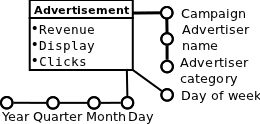
\includegraphics[scale=0.5]{fact_advertisement}
\caption{\label{pic:f_adv}  Advertisement}
\end{center}
\end{figure}

\begin{figure}[!hbp]
\begin{center}
    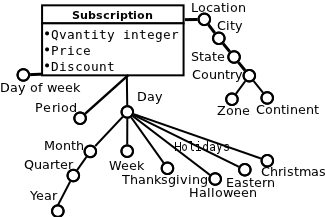
\includegraphics[scale=0.5]{fact_subscriptions}
\caption{\label{pic:f_sub}  Subscriptions}
\end{center}
\end{figure}

\begin{figure}[!hbp]
\begin{center}
  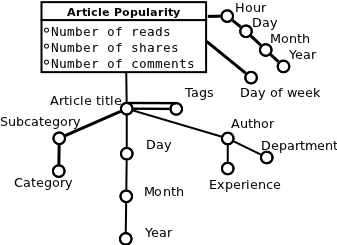
\includegraphics[scale=0.5]{fact_article}
\caption{\label{pic:f_art}  Article popularity}
\end{center}
\end{figure}


        \subsection{Fact Measures} \label{sub:ml1_measures}
        
{\bf Advertisement} fact has measures {\it Revenue},{\it Displays},{\it Clicks}. All 3 measures are additive of an integer type. All three measures could be combined to compute secondary statistic, e.g. Click rate $Clicks / Displays$. 

{\bf Subscription} is measured by {\it Price}, {\it Discount} and {\it Quantity}. The measures simply reflects the act of subscribing per one order. {\it Quantity} is number of subscriptions in one order. {\it Price} and {\it Quantity} are additive measures. {\it Discount} is proportional e.g. 0.1 meaning $10\%$ discount. It means it is not additive, however an average discount per order makes sense.

{\bf Article popularity} could be measured by {\it Number of reads}, {\it Number of shares} and {\it Number of comments}.
All three measures are additive.

All additive measures in all three facts could be sum up allong its hierachies for additional attributs. The average could be counted using {\it SUM} and {\it COUNT} on corresponding level, but realise that average of averages from disjoint subsets is not average from a the whole set.

        \subsection{Attributes and Hierarchies} \label{sub:ml1_attributes}
        

We offers different types of subscriptions based on how long the subscription last. We reflect it in attribute period.


        \subsection{Conceptual problems} \label{sub:ml1_problems}
        At first, we had difficulty identifying facts, but as we discussed business processes and made up sample business queries, we managed to identify the facts.

Secondly, we looked at facts more from a relational point of view. We did not consider evolution
of data in time, so we thought about updates in our data warehouse. Especially difficult for us was to avoid updates in facts about articles. We had originally designed the fact that had reflected only actual state. Instead of adding new information and keeping historical data, we had though about updating values in data warehouse. It was clearly wrong solution.

Finally, we managed to figure out how to designed the fact and keep the measures reads, shares and comments and also we know that the tables are sensible large.

        \clearpage
    % section Conceptual Design of Data Warehouse (end)

    \section{Logical design} 
            \label{sec:ml1_logical}
        \subsection{Star schemas} \label{sub:ml1_star}
        
\begin{figure}[!hbp]
\begin{center}
    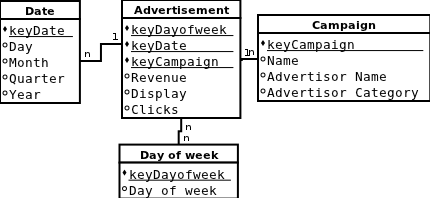
\includegraphics[scale=0.5]{schema_star_advertisement}
\caption{\label{pic:st_adv} Star schema - Advertisement}
\end{center}
\end{figure}

\begin{figure}[!hbp]
\begin{center}
    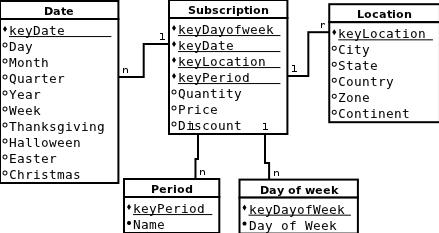
\includegraphics[scale=0.5]{schema_star_subscriptions}
\caption{\label{pic:st_sub}  Star schema - Subscriptions}
\end{center}
\end{figure}

\begin{figure}[!hbp]
\begin{center}
    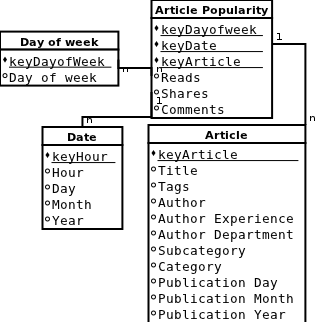
\includegraphics[scale=0.5]{schema_star_article}
\caption{\label{pic:st_art}  Star schema - Article}
\end{center}
\end{figure}


        \clearpage
        \subsection{Snowflake schemas} \label{sub:ml1_snowflake}
        
\begin{figure}[!hbp]
    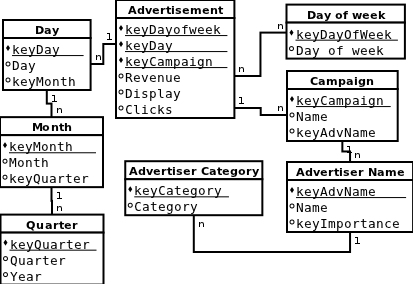
\includegraphics[scale=0.4]{schema_snowflake_advertisement}
\caption{\label{pic:sn_adv} Snowflake schema - Advertisement}
\end{figure}

\begin{figure}[!hbp]
    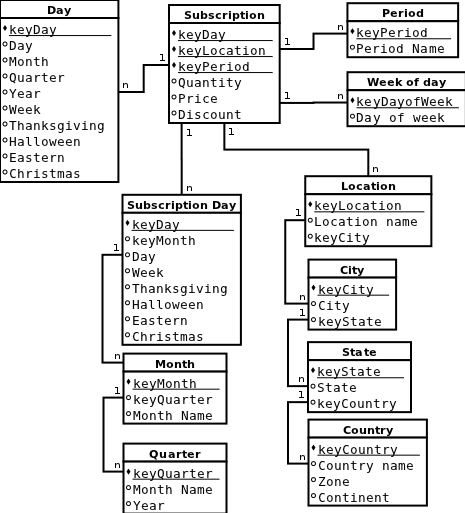
\includegraphics[scale=0.4]{schema_snowflake_subscriptions}
\caption{\label{pic:sn_sub}  Snowflake schema - Subscriptions}
\end{figure}

\begin{figure}[!hbp]
    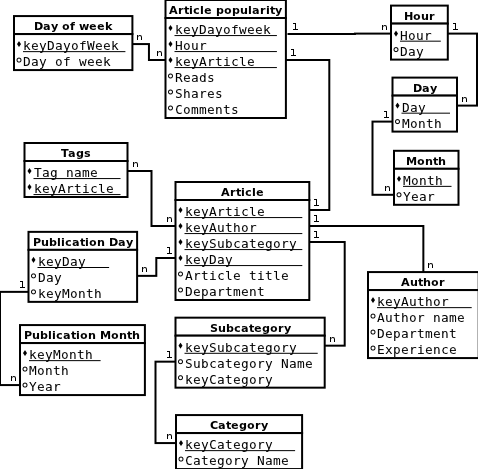
\includegraphics[scale=0.4]{schema_snowflake_article}
\caption{\label{pic:sn_art} Snowflake schema - Article}
\end{figure}

\clearpage

        \subsection{Choice between schemas} \label{sub:ml1_choice}
        
Due to the fact that our dimension tables are not so large, in sense of branching, and also they contain simple domains, the tables in star schema do not cover too much space.
 The star schema also allows better performance for data warehouse queries. In other words, the low normality of tables does not affect the space requirements too badly, because the numbers of possible values in hierarchies are relatively low.

On the other hand, the star schema allows us process aggregation function more effectively.
The aggregation functions together with joins are the key operations for data warehouse. 
The snowflake schema is in our case split in a lot of tables with relatively small number of values.
It does not save so much space compare to star schema, but only it results in sequences of joins.
To conclude, we decided to follow star schema and avoid joins in our queries as much as possible.

The only exception, which does not allow us to follow our star schema from Section~\ref{sub:ml1_star}, is the {\it Tag} attribute. 
The {\it Tag} attribute from {\it Article popularity} fact has potentially unlimited domain, because every author or editor can add arbitrary tag.  
We are using only sample data for it, but we still created a separate table for describing $n$ to $n$ relation between Tags and Articles. 
The table could be very huge and is nonsense  to make the table of {\it Article} dimension wider by another columns as it is displayed in star schema design. 

        \clearpage % for Snowflake schemas
        \subsection{Example data} \label{sub:ml1_example}
        In tables below you see sample date for a star schema introduced in~Subsection~\ref{sub:ml1_star}. As we mention in  Subsection~\ref{sub:ml1_choice} we did not used in our implementation exactly the star schema, but we separated {\it tags} attribute to another table. So notice that in our implementation we added a {\it keyTag} column in Table~\ref{t:f_artpop}, remove column {\it Tags} in  Table~\ref{t:art_dim_table} and we created {\bf separate table {\it Tags}}.
\begin{figure}[!hbp]
\caption{\label{t:f_adv}Advertisement fact table}
\begin{center}
\begin{tabular}{|c|c|c|c|c|}
\hline
keyDate & keyCampaign & Revenue & Displays & Clicks\\
\hline
\hline
874 & 32 & 20000 & 432812 & 4221\\
932 & 872 & 399 & 21322 & 213\\
\hline
\end{tabular}
\end{center}
\end{figure}

\begin{figure}[!hbp]
\caption{\label{t:adv_date}Advertisement Date dimension table}
\begin{center}
\begin{tabular}{|c|c|c|c|c|}
\hline
keyDate & Date & Month & Quarter & Year\\
\hline
\hline
874 & 23 & 1 & 1 & 2008\\
932 & 5 & 5 & 2 & 2006\\
\hline
\end{tabular}
\end{center}
\end{figure}

\begin{figure}[!hbp]
\caption{\label{t:adv_camp}Advertisement Campaign dimension table}
\begin{center}
\begin{tabular}{|c|c|c|c|}
\hline
keyCampaign & Name & Advertiser Name & Advertiser Category\\
\hline
\hline
32 & 2012 Volkswagen CC Ad & Volkswagen & Big Fish\\
872 & Free Lunch at Mensa & Bolzano University & Small Fish\\
\hline
\end{tabular}
\end{center}
\end{figure}

\begin{figure}[!hbp]
\caption{\label{t:f_sub}Subscription fact table}
\begin{center}
\begin{tabular}{|c|c|c|c|c|c|}
\hline
keyDate & keyLocation & keyPeriod & Quantity & Price & Discount\\
\hline
\hline
423 & 2311 & 1223 & 2 & 100.58 & 0.1\\
43 & 88 & 8898 & 10 & 920.3 & 0.1\\
\hline
\end{tabular}
\end{center}
\end{figure}

\begin{figure}[!hbp]
\caption{\label{t:sub_date}Subscription date dimension table}
\begin{center}
\begin{tabular}{|c|c|c|c|c|c|p{1.3cm}|p{1.2cm}|p{1.3cm}|p{1cm}|}
\hline 
keyDate &Date&Month&Quarter& Year & Week & Thanks- giving & Eastern & Christ- mas & Hallo- ween\\
\hline
\hline
423 & 31 & 10 & 4 & 2011 & 1 & 0 & 0 & 0 & 1\\
43 & 24 & 12 & 4 & 2005 & 6 & 0 & 0 & 1 & 0\\
\hline
\end{tabular}
\end{center}
\end{figure}


\begin{figure}[!hbp]
\caption{\label{t:sub_loc|}Subscription location dimension table}
\begin{center}
\begin{tabular}{|c|c|c|c|c|c|}
\hline
keyLocation & City & State & Country & Zone & Continent\\
\hline
\hline
2311 & New York & New York & United States & US and Canada & North America\\
88 & Bolzano & South Tyrol & Italy & Southern Europe & Europe\\
\hline
\end{tabular}
\end{center}
\end{figure}

\begin{figure}[!hbp]
\caption{\label{t:sub_per}Subscription period dimension table}
\begin{center}
\begin{tabular}{|c|c|c|}
\hline
keyPeriod & Name & Order\\
\hline
\hline
1223 & Month& 3\\
8898 & Annual& 5\\
\hline
\end{tabular}
\end{center}
\end{figure}

\begin{figure}[!hbp]
\caption{\label{t:f_artpop}Article Popularity fact table}
\begin{center}
\begin{tabular}{|c|c|c|c|c|}
\hline
keyDate & keyArticle & Reads & Shares & Comments\\
\hline
\hline
2011020117 & 1000 & 212 & 20 & 5\\
2011020118 & 1000 & 53 & 2 & 4\\
\hline
\end{tabular}
\end{center}
\end{figure}

\begin{figure}[!hbp]
\caption{\label{t:art_date}Article Popularity Date dimension table}
\begin{center}
\begin{tabular}{|c|c|c|c|c|}
\hline
keyDate  & Hour & Date & Month & Year\\
\hline
\hline
2011020117 & 17 & 02 & 11 & 2011\\
\hline
2011020118 & 18 & 02 & 11 & 2011\\
\hline
\end{tabular}
\end{center}
\end{figure}


\begin{figure}[!hbp]
\caption{\label{t:art_dim_table}Article Popularity dimension table }
\begin{center}
\begin{tabular}{|p{1cm}|p{1cm}|p{1cm}|p{1.25cm}|p{1.25cm}|p{1.25cm}|p{1.35cm}|p{1.3cm}|p{0.7cm}|p{1.05cm}|p{0.9cm}|}
\hline
key Article & Title & Tags & Author & Author Exp. & Author Dept. & Sub category & Cate- gory & Pub. Day & Pub. Month & Pub. Year\\
\hline
\hline
1000 & Article  & rude funny & John Smith & Junior Reporter & Enter- tainment & Fashion & Life and Style & 02 & 11 & 2011\\
\hline
9999 & Wake the economy & serious actual&Jane Doe & Senior Reporter & Finance & Earnings & Business & 03 & 11 & 2011\\
\hline
\end{tabular}
\end{center}
\end{figure}

        \clearpage
%force to print all figures
    % section Logical design (end)

    \section{SQL Implementation} % (fold)
    \label{sec:implementation}
    
Our data was generated partially randomly and partially randomly chosen from public databases.
Firstly, we created the populating scripts for PostgresSQL 9.1. Lately, we decided to migrate
our database to Oracle 10.2.0.3.0, because Postgres does not support data mining extensions.
We had to modify the populating scripts to fit Oracle syntax and also subdivide them,
because Oracle does not support some commands with our permissions, e.g. "CREATE SCHEMA" command.

We divided generated data into several SQL scripts which creates tables, populates tables, and delete tables.
We provide init.sh file. It allows to populate database, see Figure~\ref{l:ml1_init}, and also deleting the tables, see Figure~\ref{l:ml1_drop}.
\begin{figure}[!hbp]
\begin{lstlisting}[language=bash]
$ cd init
# comment: init connects to database granted to us from school
# comment: for more information check the script itself
$ ./init.sh init login password
# it will take quite about 4 hours to populate the data
\end{lstlisting}
\caption{Populating data warehouse using  init.sh script} \label{l:ml1_init}
\end{figure}

\begin{figure}[!hbp]
\begin{lstlisting}[language=bash]
$ cd init
# comment: droping the table/ removing the data warehouse 
# comment: still from init directory
$ ./init.sh drop login password
\end{lstlisting}
\caption{Removing data warehouse using  init.sh script} \label{l:ml1_drop}
\end{figure}

For more details about SQL scripts, the init.sh script or the script for generating data view the source code of the scripts, it should be self explenatory. In enclosed README.txt we list all containing scripts and the usage again.

\subsection*{Data}
To generate the SQL scripts for populating the database we used PHP scripts enclosed.

We created some data artificially, for some we used real world data.
It is worth to note that we used real address data from Canada and also we filled the tags with a few samples from real tags from real Wall Street Journal.

% subsection Data (end)


% chapter Milestone 1 (end)

\chapter{Milestone - Data warehouse querying} \label{cha:ml2}
    \section{Content of Milestone~\ref{cha:ml2}} 
        \label{sec:ml2_content}
    
\subsection*{Task} % (fold)
\label{sub:name}
For the designed data warehouse write 20 aggregation queries in both natural language and SQL. Include the results (if the resulting data amount is big, include a sample).
% subsection Task (end)


    \section{Business queries} \label{sec:Business queries}
    \section{Business queries} % (fold)
\label{sub:Business queries}

\subsection*{Task} % (fold)
\label{sub:name}
For the designed data warehouse write 20 aggregation queries in both natural language and SQL. Include the results (if the resulting data amount is big, include a sample).
% subsection Task (end)

\subsection*{Subscription queries} % (fold)
\label{sub:Subscription business queries}
\begin{enumerate}
  \item Revenue from subscriptions by year.
\begin{lstlisting}[language=sql]
select sum(price * (1-discount) * quantity) revenue, d.year 
from sub_subscription s 
join sub_date d on s.keydate = d.keydate 
group by d.year 
order by year desc
\end{lstlisting}
  \item Which were the most popular subscription periods each year?
\begin{lstlisting}[language=sql]
select year, p.name as period, sum(quantity) subscriptions
from oplatek.sub_subscription s 
join oplatek.sub_date d on s.keydate = d.keydate
join oplatek.sub_period p on s.keyperiod = p.keyperiod 
group by d.year, p.name
order by year desc, subscriptions desc
\end{lstlisting}
  \item Revenue from subscriptions and subscription count by country in 2010.
\begin{lstlisting}[language=sql]
select l.country, sum(price * (1-discount) * quantity) revenue, 
  sum(quantity) subscriptions 
from oplatek.sub_subscription s 
join oplatek.sub_location l on s.keylocation = l.keylocation 
join oplatek.sub_date d on s.keydate = d.keydate and d.year = 2010
group by l.country 
order by revenue desc
\end{lstlisting}
  \item Top 10 cities from each country with the highest revenue from subscriptions in 2010.
\begin{lstlisting}[language=sql]  
select * from (select country, city, 
  sum(price * (1-discount) * quantity) revenue, 
  rank() over(partition by country 
    order by sum(price * (1-discount) * quantity) desc) rank 
from oplatek.sub_subscription s 
join oplatek.sub_date d 
  on s.keydate = d.keydate and d.year = 2010
join oplatek.sub_location l 
  on s.keylocation = l.keylocation
group by l.country, l.city
order by revenue desc)
where rank <= 10
\end{lstlisting}
  \item How much would we earn without applying discounts on subscriptions, by period type and by year?
\begin{lstlisting}[language=sql] 
select year, period, revenue, revenue_no_discounts, 
  (revenue_no_discounts - revenue) difference from 
    (select d.year, p.name as period, 
      sum(price * (1-discount) * quantity) revenue, 
      sum(price * quantity) revenue_no_discounts
     from oplatek.sub_subscription s 
     join oplatek.sub_date d on s.keydate = d.keydate
     join oplatek.sub_period p on s.keyperiod = p.keyperiod
     group by d.year, p.name)
order by year desc, period asc
\end{lstlisting}
  \item Number of sales on different holidays by period in Canada in 2010.
\begin{lstlisting}[language=sql] 
TODO
select country, year, period, total_sales, 
(select sum(quantity) from 
    oplatek.sub_subscription ss, oplatek.sub_date dd 
 where ss.keydate = dd.keydate and dd.christmas = 'Y' 
  and ss.keyperiod = p.keyperiod 
  and ss.keylocation = l.keylocation) as christmas,
 from (select l.country, d.year, p.name period, sum(quantity) total_sales
 from oplatek.sub_subscription s 
 join oplatek.sub_date d on s.keydate = d.keydate and d.year = 2010
 join oplatek.sub_location l on s.keylocation = l.keylocation and l.country = 'Canada'
 join oplatek.sub_period p on s.keyperiod = p.keyperiod 
 group by l.country, d.year, p.name)
order by d.year, period
\end{lstlisting}
  \item Revenue by month and by state in Canada in 2010 together with average revenue by states in Canada in the same month.
\begin{lstlisting}[language=sql] 
select l.state, d.month, 
  sum(price * (1-discount) * quantity) revenue,
  /* avg_revenue_in_this_month_across_all_states */
  avg(sum(price * (1-discount) * quantity)) 
    over (partition by month) avg_rev 
from oplatek.sub_subscription s 
join oplatek.sub_location l 
    on s.keylocation = l.keylocation and l.country = 'Canada' 
join oplatek.sub_date d 
    on s.keydate = d.keydate and d.year = 2010
where length(l.state) = 2
group by l.state, d.month
order by state asc, month asc
\end{lstlisting}
\end{enumerate}
% subsection Subscription queries (end)

\subsection*{Article queries} % (fold)
\label{sub:Article  queries}
\begin{enumerate}
\item    Top 10 read articles and their authors for every month in year 2011.
\begin{lstlisting}[language=sql] 
select * from (
 select d.month, a.keyarticle as id, 
  a.title, a.author, sum(reads) reads, 
  rank() over (partition by month order by sum(reads) desc) rank 
 from oplatek.artpop_articlepopularity f
 join oplatek.artpop_article a on f.keyarticle = a.keyarticle
 join oplatek.artpop_date d on f.keydate = d.keydate 
     and d.year = 2010
 group by d.month, a.keyarticle, a.title, a.author
 order by month asc, reads desc
) where rank <= 10
\end{lstlisting}
\item    Hours of the day when most articles are read grouped by category in year 2010 together with the average number of articles read during this hour in the same year.
\begin{lstlisting}[language=sql] 
select a.category, d.hour, sum(reads) reads, 
    avg(sum(reads)) over (partition by hour) avg_reads 
from oplatek.artpop_articlepopularity f
join oplatek.artpop_article a on f.keyarticle = a.keyarticle
join oplatek.artpop_date d on f.keydate = d.keydate 
    and d.year = 2010
group by a.category, d.hour
order by a.category asc, d.hour asc
\end{lstlisting}
\item    Number of articles published in each subcategory in year 2010 together with the % of total articles in the category.
\begin{lstlisting}[language=sql] 
select category, subcategory, articles/sum(articles) over (partition by category) perct, articles, sum(articles) over (partition by category) as articles_in_category from (
select a.category, a.subcategory, count(a.keyarticle) articles
from oplatek.artpop_articlepopularity f
join oplatek.artpop_article a on f.keyarticle = a.keyarticle and a.publicationyear = 2011
group by a.category, a.subcategory
order by category, subcategory
)
\end{lstlisting}
\item    Top 5 authors in every category by comments on their articles.
\begin{lstlisting}[language=sql] 
select * from (
select a.category, a.author, sum(comments) comments, 
  rank() over (partition by a.category 
    order by sum(comments) desc) rank 
from oplatek.artpop_articlepopularity f
join oplatek.artpop_article a on f.keyarticle = a.keyarticle
group by a.category, a.author
order by a.category asc, comments desc
) where rank <= 5
\end{lstlisting}
\item    Each author's 5 most read articles with the number of total article reads together with the average number of article reads for this author's department and each author must have at least 20 articles published, all these articles must have been published before 2011 and total reads for each article must be above the average article read count for the author's department.
\begin{lstlisting}[language=sql] 
select *
from (select a.author, 
  rank() 
    over (partition by a.author order by sum(reads) desc) rank,
  a.keyarticle id, a.title,
  sum(reads) reads, 
  a.authordepartment department,
  avg(sum(reads)) 
    over (partition by a.authordepartment) deparment_reads,
  count(a.keyarticle) 
    over (partition by a.author) total_articles
from oplatek.artpop_articlepopularity f
join oplatek.artpop_article a on f.keyarticle = a.keyarticle
where a.publicationyear < 2011
group by a.author, a.authordepartment, a.keyarticle, a.title
order by a.author, rank asc)
where rank <= 5 and reads > deparment_reads 
and total_articles >= 20
\end{lstlisting}
\item    Top 20 articles published in October, 2011 with the \#comments/\#reads higher than the average \#comments/\#reads having at least 20000 \#reads.
\begin{lstlisting}[language=sql] 
select * from (
select a.keyarticle id, a.title,
   sum(reads)/sum(comments) comm_by_reads,
   avg(sum(reads)/sum(comments)) over () avg_comm_by_reads,
   sum(reads) reads
from oplatek.artpop_articlepopularity f
join oplatek.artpop_article a on f.keyarticle = a.keyarticle
where a.publicationyear = 2011 
and a.publicationmonth = 10
group by a.keyarticle, a.title
order by comm_by_reads - avg_comm_by_reads desc
) where comm_by_reads > avg_comm_by_reads 
and reads >= 20000 and rownum <= 20
\end{lstlisting}
\item    Compare the number of reads/shares/comments of articles tagged with positive and negative tags for each year.
\begin{lstlisting}[language=sql] 
select year, tag, 
reads, sum(reads) over (partition by year) reads_total, reads/sum(reads) over (partition by year) reads_perc,
reads, sum(shares) over (partition by year) shares_total, shares/sum(shares) over (partition by year) shares_perc,
reads, sum(comments) over (partition by year) comments_total, comments/sum(comments) over (partition by year) comments_perc
from (
select a.publicationyear year, t.tag, sum(reads) reads, sum(comments) comments, sum(shares) shares
from oplatek.artpop_articlepopularity f
join oplatek.artpop_article a on f.keyarticle = a.keyarticle
join oplatek.artpop_tag t on t.tag in ('positive', 'negative')
join oplatek.artpop_articletags artt on a.keyarticle = artt.keyarticle and artt.keytag = t.keytag 
group by a.publicationyear, t.tag
order by year desc, tag
)
\end{lstlisting}
\item   Top 100 tags by article count in Business category in 2011.
\begin{lstlisting}[language=sql] 
select rank() over (order by count(a.keyarticle) desc) rank, t.tag, count(a.keyarticle) articles
from oplatek.artpop_articlepopularity f
join oplatek.artpop_article a on f.keyarticle = a.keyarticle and a.category = 'Business' and a.publicationyear = 2011
join oplatek.artpop_tag t on 1=1
join oplatek.artpop_articletags artt on a.keyarticle = artt.keyarticle and artt.keytag = t.keytag
group by t.tag
order by rank, tag asc
\end{lstlisting}
\end{enumerate}
% subsection Article  queries (end)

\subsection*{Advertisement  queries} % (fold)
\label{sub:Advertisement queries}

\begin{enumerate}
\item    Revenue by year together with average revenue in all years together with revenue in this year and together with next year
\begin{lstlisting}[language=sql] 
select ad.Year, sum(aa.revenue), 
  avg(sum(aa.revenue)) over () as total_avg,
  sum(sum(aa.revenue)) over 
    (order by ad.year rows 1 preceding) as sum_last_2_years
from   
advert_advertisement aa
join advert_date ad on aa.keydate = ad.keydate
group by ad.YEAR;
  \end{lstlisting}
\item    CPM(Clicks divided by displays) for top 10 advertisers by revenue together with avg CPM for advertisers category having the advertiser at least 15 campaigns
  \begin{lstlisting}[language=sql] 
select *
from 
(    select
        rank() over (order by sum (aa.revenue) desc) as top,
        sum(aa.clicks)/sum(aa.displays),ac.advertiserName,
        ac.advertiserCategory as cat, 
        avg(sum(aa.clicks)/sum(aa.displays)) 
            over (partition by ac.advertiserCategory)
    from advert_advertisement aa
    join advert_campaign ac on aa.keycampaign = ac.keycampaign
    join
      ( select distinct in_aa.advertiserName 
        from advert_campaign in_aa
        group by in_aa.advertiserName
        having COUNT(in_aa.name) >= 15
      )
    camp on ac.advertiserName = camp.advertiserName
    group by rollup (ac.advertiserName,ac.advertiserCategory) 
    having grouping_id(ac.advertiserName,ac.advertiserCategory)=0
    )
where 
top < 10;
\end{lstlisting}
\item Revenue by advertiser from "Small Fish" category who has greater revenue than average of the "Middle Fish"*bias=0.5 together with average of "Middle Fish" advertisers  
  \begin{lstlisting}[language=sql] 
select ac.advertiserName, ac.advertiserCategory, sum(aa.revenue), 
 avg(sum(aa.revenue)) over (partition by ac.advertiserCategory) 
 as small_fish_avg,
 ( 
  select distinct
   AVG(sum(aaa.revenue)) over 
    (partition by aac.advertiserCategory) as middle_fish_avg
    from advert_advertisement aaa 
    join advert_campaign aac on aaa.keycampaign = aac.keycampaign
    where aac.advertiserCategory = 'Medium Fish'   
    group by aac.advertiserName,aac.advertiserCategory
  ) as middle_fish_avg
from advert_advertisement aa
join advert_campaign ac on aa.keycampaign = ac.keycampaign
where ac.advertiserCategory = 'Small Fish'
group by ac.advertiserName,ac.advertiserCategory
having sum(aa.revenue) > 0.5* (
  -- having is stupid, I have to repeat query:)
  select distinct
    AVG(sum(aaa.revenue)) over (partition by aac.advertiserCategory) 
    as middle_fish_avg
  from advert_advertisement aaa 
  join advert_campaign aac on aaa.keycampaign = aac.keycampaign
  where aac.advertiserCategory = 'Medium Fish'   
  group by aac.advertiserName,aac.advertiserCategory);
  \end{lstlisting}
\item    The Campaigns which touched more than 5 month with maximum revenue in one month bigger than 140 all in year 2011 
  \begin{lstlisting}[language=sql] 
select * from (
  select ac.name, max(sum(aa.revenue)) 
    over (partition by ac.name) as max_revenue_over_month
  from advert_advertisement aa
  join advert_date ad on ad.keyDate = aa.keyDate
  join advert_campaign ac on ac.keyCampaign = aa.keyCampaign
  where ad.year=2011
  group by ac.name, ad.month
  having ( max(ad.month) - min(ad.month)) >= 0 
    or ( (max(ad.month) - min(ad.month)) = 5 
    and (max(ad.day) - min(ad.day)) >=0 )
) where max_revenue_over_month > 140;
  \end{lstlisting}
\item Most popular campaigns by year together with their popularity(clicks+displays) and  avg CPM per month
  \begin{lstlisting}[language=sql] 
select y, c, n, popularity, cpm_per_month
from (
  select ad.year y, ac.name n,  ad.month, ac.advertisercategory c
  , sum(aa.clicks+aa.displays) popularity
  ,(avg(sum(aa.clicks)/sum(aa.displays)) 
    over (partition by ad.month)) cpm_per_month 
  from advert_advertisement aa
  join advert_date ad on ad.keyDate = aa.keyDate
  join advert_campaign ac on ac.keyCampaign = aa.keyCampaign
  group by ad.month,ad.year, ac.name,ac.advertisercategory
  )
order by y desc, c, popularity desc, n;

  \end{lstlisting}
\end{enumerate}
% section Business queries (end)

% section Advertisement business queries (end)


% chapter Milestone 2 (end)

\chapter{Milestone 3} \label{cha:ml3}
    \section{Content of Milestone~\ref{cha:ml3}} 
        \label{sec:ml3_content}
    The main purpose of this milestone is to try out various data mining techniques.

We decided to explore the following data mining techniques in this milestone: classification, prediction and clustering. For each technique we evaluated various algorithms mentioned in the lectures and compared them to some others that were available to use in the data mining software package that we used. 

We also extracted some new information from the models built during the mining process to show some things that we found interesting which is also the goal of the MSR 2012 challange.

\section{Data} % (fold)
\label{sub:Data}
We chose to mine the Android bug database because it was the data was already provided by the organizers of the MSR 2012 challange. More specifically, we chose to focus on the bug reports in this database as we believe it is the most important part of the entire database and it should give the most interesting results. The database contains 20169 reported bugs (up to December 3, 2011). 

\subsection*{Description of the data} % (fold)
\label{sub:Description of the data}

Here is the available data about the bugs.

\begin{itemize}
\item Bug ID - unique identifier assigned to each bug
\item Title - short description of the bug
\item Description - detailed description of the bug without a predefined structure
\item Type - type of the bug: Defect (bug report), Enhancement (feature request)
\item Status - current status of the bug (Reviewed, New, Duplicate, Declined, NeedsInfo, FutureRelease, Released, Spam, Unreproducible, Question, WorkingAsIntended, Assigned, Unassigned, UserError)
\item Priority - urgency of the bug to be fixed (Small, Medium, High, Critical, Blocker)
\item Component - category of the bug based on which part of the system the bug affects
\item Stars - number of people that have starred this bug (could be an indicator of popularity)
\item Owner - assigned developer to fix  the bug
\item Reported By - person who reported the bug
\item Opened Date - when the bug was reported
\item Closed On - when the bug was marked as closed
\end{itemize}

It is also possible to aggregate the comments for a bug to determine additional data about it.

\begin{itemize}
\item Comment count - the number of comments for this bug
\item Number of commenters - the number of distinct people participating in the discussion about the bug
\item How long it took the solve the bug - by subtracting the close date from the open date
\end{itemize}

Title, description, type are entered by the user. System also automatically generated the bug id, marks it as a new bug, assigns a medium priority to the bug, makes the user as the reporter of the bug and sets the opened date to the date and time of the submition.

Component and owner are later manually assigned by one of the administrators. Status, priority can later be changed, however, these changes are not reflected in the available data, only the latest state of the bug is available.
% subsection Description of the data (end)

\subsection*{Processing of the data} % (fold)

The bug database which was provided as a single XML file was converted to a CSV file using a manually written script which contains all bug properties, previously mentioned aggregated properties but doesn't contain any of the comments.

This CSV file was later imported in the data mining software package that we used and each property was assigned a type as seen in the screenshot below. In this particular case shown in the screenshot, *Component* was selected as the label or class for classification.

*s1\_types.png*

Properties of type *text* will be later converted to vectors using the text processing features of the data mining software package.

% subsection Processing of the data (end)

% section Data (end)

\section{Tools} % (fold)
\label{sub:Tools}

\subsection{Weka} % (fold)
\label{sub:Weka}

At first we used the tool Weka to familiarise ourselves with ....

% subsection Weka (end)

\subsection{Rapid Miner} % (fold)
\label{sub:Rapid Miner}

Our tool of choice was Rapid Miner because ...

% subsection Rapid Miner (end)

% section Tools (end)

\section{Classification} % (fold)
\label{sub:Classification}

\subsection{Classification of bugs by component} % (fold)
\label{sub:Classification of bugs bugs by component}

When a bug report is submitted, someone has to look at it and determine which component it affects and assigned an appropriate label. Currently it is done manually by one of the maintainers. We wondered if it's possible to use data mining to automatically classify new bugs by component.

We came to the conclusion that only title and description should be used to determine the component since they describe the bug but other properties are just metadata. The outcome of the classifier should be the component name that this bug affects.

Only the bugs which already had a component label assigned to them were chosen as the training data for data mining because the bugs with a component assigned to them are already classified and we didn't have to do it manually.

Title and description values were transformed into lower case and then tokenized using non letters as delimiters and then word vectors were generated from them using TF-IDF. It's worth pointing out that if a more sophisticated tokenization algorithm was used, perhaps it would significantly improve the accuracy of classifiers.

After the data was pre-processed, we chose various classifying algorithms that were learned about in class and compared their accuracy. Accuracy is used to assess the performance of classifiers. It was mentioned in the lectures that a stratified 10-fold cross validation is recommended for estimating accuracy. Because we wanted to try out various algorithms and compare them, we only used a sample of data because it would take too much time to the classifiers to run on our desktop computers.

Type             Algorithm     Sample    Time    Accuracy
Decision Trees   Weka J48       500      2:19      44.80%
Decision Trees   Weka J48      1000     10:25      45.50%
Decision Trees   Weka LAD-Tree  500       

% subsection Classification of bugs bugs by component (end)

\subsection{Classification of bugs by developer} % (fold)
\label{sub:Classification of bugs bugs by developer}
% subsection Classification of bugs bugs by developer (end)

% section Classification (end)

\section{Prediction} % (fold)
\label{sub:Prediction}

\subsection{Prediction of bug lifespan} % (fold)
\label{sub:Prediction of bug lifespan}
% subsection Prediction of bug lifespan (end)

\section{Clustering} % (fold)
\label{sub:Clustering}
% section Clustering (end)

\section{Test} % (fold)
\label{sec:Test}

% section Test (end)



% chapter Milestone 3 (end)

%do not remove!
\end{document}

